% Options for packages loaded elsewhere
% Options for packages loaded elsewhere
\PassOptionsToPackage{unicode}{hyperref}
\PassOptionsToPackage{hyphens}{url}
\PassOptionsToPackage{dvipsnames,svgnames,x11names}{xcolor}
%
\documentclass[
  letterpaper,
  DIV=11,
  numbers=noendperiod]{scrartcl}
\usepackage{xcolor}
\usepackage{amsmath,amssymb}
\setcounter{secnumdepth}{-\maxdimen} % remove section numbering
\usepackage{iftex}
\ifPDFTeX
  \usepackage[T1]{fontenc}
  \usepackage[utf8]{inputenc}
  \usepackage{textcomp} % provide euro and other symbols
\else % if luatex or xetex
  \usepackage{unicode-math} % this also loads fontspec
  \defaultfontfeatures{Scale=MatchLowercase}
  \defaultfontfeatures[\rmfamily]{Ligatures=TeX,Scale=1}
\fi
\usepackage{lmodern}
\ifPDFTeX\else
  % xetex/luatex font selection
\fi
% Use upquote if available, for straight quotes in verbatim environments
\IfFileExists{upquote.sty}{\usepackage{upquote}}{}
\IfFileExists{microtype.sty}{% use microtype if available
  \usepackage[]{microtype}
  \UseMicrotypeSet[protrusion]{basicmath} % disable protrusion for tt fonts
}{}
\makeatletter
\@ifundefined{KOMAClassName}{% if non-KOMA class
  \IfFileExists{parskip.sty}{%
    \usepackage{parskip}
  }{% else
    \setlength{\parindent}{0pt}
    \setlength{\parskip}{6pt plus 2pt minus 1pt}}
}{% if KOMA class
  \KOMAoptions{parskip=half}}
\makeatother
% Make \paragraph and \subparagraph free-standing
\makeatletter
\ifx\paragraph\undefined\else
  \let\oldparagraph\paragraph
  \renewcommand{\paragraph}{
    \@ifstar
      \xxxParagraphStar
      \xxxParagraphNoStar
  }
  \newcommand{\xxxParagraphStar}[1]{\oldparagraph*{#1}\mbox{}}
  \newcommand{\xxxParagraphNoStar}[1]{\oldparagraph{#1}\mbox{}}
\fi
\ifx\subparagraph\undefined\else
  \let\oldsubparagraph\subparagraph
  \renewcommand{\subparagraph}{
    \@ifstar
      \xxxSubParagraphStar
      \xxxSubParagraphNoStar
  }
  \newcommand{\xxxSubParagraphStar}[1]{\oldsubparagraph*{#1}\mbox{}}
  \newcommand{\xxxSubParagraphNoStar}[1]{\oldsubparagraph{#1}\mbox{}}
\fi
\makeatother

\usepackage{color}
\usepackage{fancyvrb}
\newcommand{\VerbBar}{|}
\newcommand{\VERB}{\Verb[commandchars=\\\{\}]}
\DefineVerbatimEnvironment{Highlighting}{Verbatim}{commandchars=\\\{\}}
% Add ',fontsize=\small' for more characters per line
\usepackage{framed}
\definecolor{shadecolor}{RGB}{241,243,245}
\newenvironment{Shaded}{\begin{snugshade}}{\end{snugshade}}
\newcommand{\AlertTok}[1]{\textcolor[rgb]{0.68,0.00,0.00}{#1}}
\newcommand{\AnnotationTok}[1]{\textcolor[rgb]{0.37,0.37,0.37}{#1}}
\newcommand{\AttributeTok}[1]{\textcolor[rgb]{0.40,0.45,0.13}{#1}}
\newcommand{\BaseNTok}[1]{\textcolor[rgb]{0.68,0.00,0.00}{#1}}
\newcommand{\BuiltInTok}[1]{\textcolor[rgb]{0.00,0.23,0.31}{#1}}
\newcommand{\CharTok}[1]{\textcolor[rgb]{0.13,0.47,0.30}{#1}}
\newcommand{\CommentTok}[1]{\textcolor[rgb]{0.37,0.37,0.37}{#1}}
\newcommand{\CommentVarTok}[1]{\textcolor[rgb]{0.37,0.37,0.37}{\textit{#1}}}
\newcommand{\ConstantTok}[1]{\textcolor[rgb]{0.56,0.35,0.01}{#1}}
\newcommand{\ControlFlowTok}[1]{\textcolor[rgb]{0.00,0.23,0.31}{\textbf{#1}}}
\newcommand{\DataTypeTok}[1]{\textcolor[rgb]{0.68,0.00,0.00}{#1}}
\newcommand{\DecValTok}[1]{\textcolor[rgb]{0.68,0.00,0.00}{#1}}
\newcommand{\DocumentationTok}[1]{\textcolor[rgb]{0.37,0.37,0.37}{\textit{#1}}}
\newcommand{\ErrorTok}[1]{\textcolor[rgb]{0.68,0.00,0.00}{#1}}
\newcommand{\ExtensionTok}[1]{\textcolor[rgb]{0.00,0.23,0.31}{#1}}
\newcommand{\FloatTok}[1]{\textcolor[rgb]{0.68,0.00,0.00}{#1}}
\newcommand{\FunctionTok}[1]{\textcolor[rgb]{0.28,0.35,0.67}{#1}}
\newcommand{\ImportTok}[1]{\textcolor[rgb]{0.00,0.46,0.62}{#1}}
\newcommand{\InformationTok}[1]{\textcolor[rgb]{0.37,0.37,0.37}{#1}}
\newcommand{\KeywordTok}[1]{\textcolor[rgb]{0.00,0.23,0.31}{\textbf{#1}}}
\newcommand{\NormalTok}[1]{\textcolor[rgb]{0.00,0.23,0.31}{#1}}
\newcommand{\OperatorTok}[1]{\textcolor[rgb]{0.37,0.37,0.37}{#1}}
\newcommand{\OtherTok}[1]{\textcolor[rgb]{0.00,0.23,0.31}{#1}}
\newcommand{\PreprocessorTok}[1]{\textcolor[rgb]{0.68,0.00,0.00}{#1}}
\newcommand{\RegionMarkerTok}[1]{\textcolor[rgb]{0.00,0.23,0.31}{#1}}
\newcommand{\SpecialCharTok}[1]{\textcolor[rgb]{0.37,0.37,0.37}{#1}}
\newcommand{\SpecialStringTok}[1]{\textcolor[rgb]{0.13,0.47,0.30}{#1}}
\newcommand{\StringTok}[1]{\textcolor[rgb]{0.13,0.47,0.30}{#1}}
\newcommand{\VariableTok}[1]{\textcolor[rgb]{0.07,0.07,0.07}{#1}}
\newcommand{\VerbatimStringTok}[1]{\textcolor[rgb]{0.13,0.47,0.30}{#1}}
\newcommand{\WarningTok}[1]{\textcolor[rgb]{0.37,0.37,0.37}{\textit{#1}}}

\usepackage{longtable,booktabs,array}
\usepackage{calc} % for calculating minipage widths
% Correct order of tables after \paragraph or \subparagraph
\usepackage{etoolbox}
\makeatletter
\patchcmd\longtable{\par}{\if@noskipsec\mbox{}\fi\par}{}{}
\makeatother
% Allow footnotes in longtable head/foot
\IfFileExists{footnotehyper.sty}{\usepackage{footnotehyper}}{\usepackage{footnote}}
\makesavenoteenv{longtable}
\usepackage{graphicx}
\makeatletter
\newsavebox\pandoc@box
\newcommand*\pandocbounded[1]{% scales image to fit in text height/width
  \sbox\pandoc@box{#1}%
  \Gscale@div\@tempa{\textheight}{\dimexpr\ht\pandoc@box+\dp\pandoc@box\relax}%
  \Gscale@div\@tempb{\linewidth}{\wd\pandoc@box}%
  \ifdim\@tempb\p@<\@tempa\p@\let\@tempa\@tempb\fi% select the smaller of both
  \ifdim\@tempa\p@<\p@\scalebox{\@tempa}{\usebox\pandoc@box}%
  \else\usebox{\pandoc@box}%
  \fi%
}
% Set default figure placement to htbp
\def\fps@figure{htbp}
\makeatother





\setlength{\emergencystretch}{3em} % prevent overfull lines

\providecommand{\tightlist}{%
  \setlength{\itemsep}{0pt}\setlength{\parskip}{0pt}}



 


\KOMAoption{captions}{tableheading}
\makeatletter
\@ifpackageloaded{caption}{}{\usepackage{caption}}
\AtBeginDocument{%
\ifdefined\contentsname
  \renewcommand*\contentsname{Table of contents}
\else
  \newcommand\contentsname{Table of contents}
\fi
\ifdefined\listfigurename
  \renewcommand*\listfigurename{List of Figures}
\else
  \newcommand\listfigurename{List of Figures}
\fi
\ifdefined\listtablename
  \renewcommand*\listtablename{List of Tables}
\else
  \newcommand\listtablename{List of Tables}
\fi
\ifdefined\figurename
  \renewcommand*\figurename{Figure}
\else
  \newcommand\figurename{Figure}
\fi
\ifdefined\tablename
  \renewcommand*\tablename{Table}
\else
  \newcommand\tablename{Table}
\fi
}
\@ifpackageloaded{float}{}{\usepackage{float}}
\floatstyle{ruled}
\@ifundefined{c@chapter}{\newfloat{codelisting}{h}{lop}}{\newfloat{codelisting}{h}{lop}[chapter]}
\floatname{codelisting}{Listing}
\newcommand*\listoflistings{\listof{codelisting}{List of Listings}}
\makeatother
\makeatletter
\makeatother
\makeatletter
\@ifpackageloaded{caption}{}{\usepackage{caption}}
\@ifpackageloaded{subcaption}{}{\usepackage{subcaption}}
\makeatother
\usepackage{bookmark}
\IfFileExists{xurl.sty}{\usepackage{xurl}}{} % add URL line breaks if available
\urlstyle{same}
\hypersetup{
  pdftitle={Class, Homeownership, and Support for Clean Energy Policy: Evidence from the 2024 CES},
  colorlinks=true,
  linkcolor={blue},
  filecolor={Maroon},
  citecolor={Blue},
  urlcolor={Blue},
  pdfcreator={LaTeX via pandoc}}


\title{Class, Homeownership, and Support for Clean Energy Policy:
Evidence from the 2024 CES}
\author{}
\date{}
\begin{document}
\maketitle


\subsection{Motivation and Question}\label{motivation-and-question}

Public support for clean energy and environmental regulation is often
described in ideological or partisan terms. While political orientation
is clearly important, less attention has been paid to how material
position, particularly in terms of housing tenure, may independently
structure climate policy attitudes.

In what follows, I explore whether homeownership predicts support for
clean energy policies after controling for the factors that are often
thought as determining such suuport: political party affiliation,
politcal ideology, and income.

Using nationally representative survey data from the 2024 Cooperative
Election Study (CES), I show that homeownership is associated with lower
support for clean energy policies even after accounting for political
orientation and standard socioeconomic controls. This pattern suggests
that climate attitudes may reflect not only ideology, but also
individuals' positions within housing and asset structures that shape
exposure to regulation and perceived costs.

\begin{Shaded}
\begin{Highlighting}[]
\ImportTok{import}\NormalTok{ os}
\NormalTok{os.getcwd()}

\NormalTok{PROJECT\_ROOT }\OperatorTok{=} \StringTok{"/Users/bradykennedy/Documents/GitHub/ClassAndClimate"}
\NormalTok{os.chdir(PROJECT\_ROOT)}
\BuiltInTok{print}\NormalTok{(}\StringTok{"Working directory set to:"}\NormalTok{, os.getcwd())}

\ImportTok{from}\NormalTok{ IPython.display }\ImportTok{import}\NormalTok{ Image, display, HTML}
\end{Highlighting}
\end{Shaded}

\begin{verbatim}
Working directory set to: /Users/bradykennedy/Documents/GitHub/ClassAndClimate
\end{verbatim}

\subsection{Data and Variables}\label{data-and-variables}

This analysis uses the 2024 CES Common Content, which is weighted to
approximate national representativeness. After cleaning the key
variables, the sample used in the final analysis includes about 56,000
respondents.

The primary outcome variable for my analysis is clean\_energy\_support,
a composite index designed to capture support for a range of
environmental and clean energy policies. This variable is constructed as
the mean of multiple binary variables taken as outcomes from the CES
survey, including support for:

-EPA regulation of carbon dioxide emissions

-Renewable electricity generation requirements

-Strengthened enforcement of the Clean Air and Clean Water Acts

-Restrictions on fossil fuel expansion and new oil and gas leases

The variable ranges from 0 to 1, with higher values indicating stronger
overall support for clean energy and environmental regulation.

\subsection{Descriptive Patterns: Income, Homeownership, and Clean
Energy
Support}\label{descriptive-patterns-income-homeownership-and-clean-energy-support}

Figure 1 presents weighted mean levels of clean energy support by income
group and homeownership status.

\begin{Shaded}
\begin{Highlighting}[]
\NormalTok{display(Image(filename}\OperatorTok{=}\StringTok{"exports/figures/clean\_energy\_by\_income\_homeowner.png"}\NormalTok{))}
\end{Highlighting}
\end{Shaded}

\pandocbounded{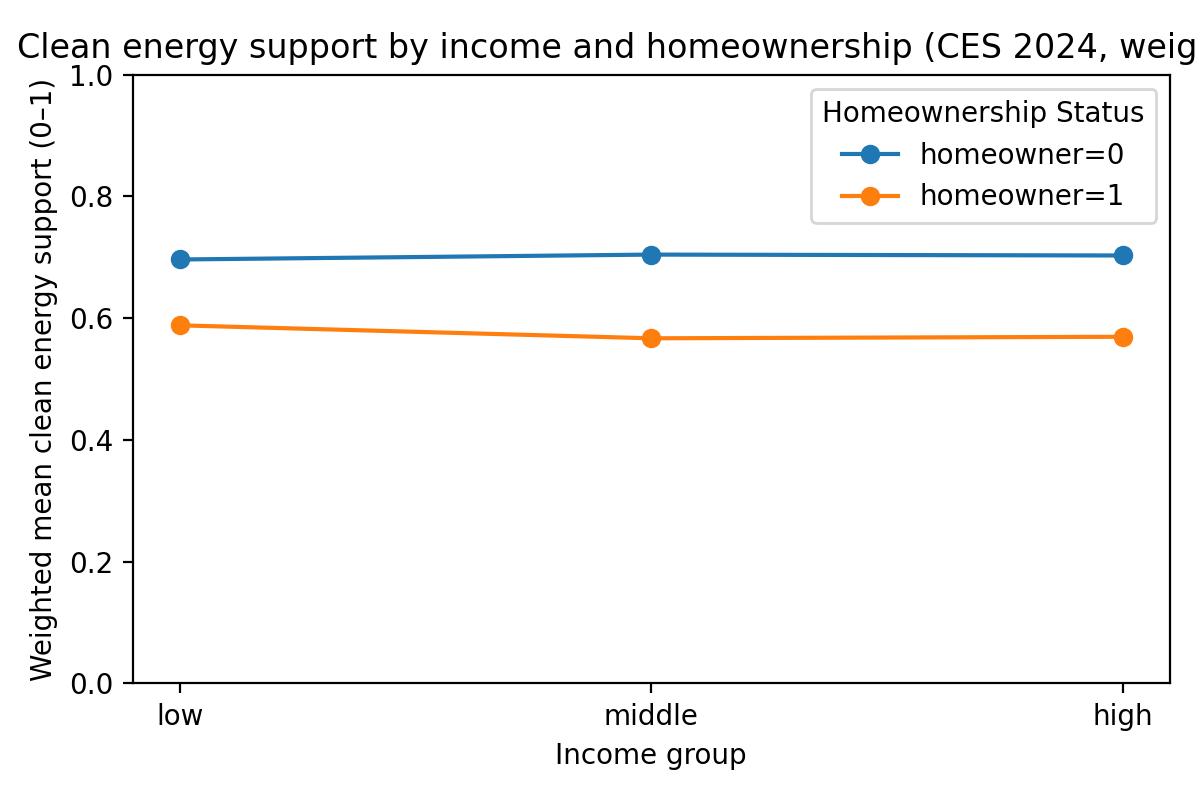
\includegraphics[keepaspectratio]{02_brief_files/figure-pdf/cell-3-output-1.png}}

Two patterns stand out from this graph. Renters exhibit consistently
higher support for clean energy policies than homeowners, across all
income groups, and income differences within tenure groups are
relatively small, especially among renters. Among renters, support for
clean energy policies is high (approximately 0.70 on a 0--1 scale)
regardless of income. Among homeowners, support is substantially lower
(roughly 0.57--0.59), again with little variation by income. These
patterns suggest that housing tenure may be more strongly associated
with climate attitudes than income alone, as will be explored further
below.

\subsection{Weighted OLS Results: Does Homeownership Matter Net of
Politics?}\label{weighted-ols-results-does-homeownership-matter-net-of-politics}

To assess whether the observed tenure gap reflects political sorting, I
estimate a weighted least squares (WLS) regression of clean energy
support on:

-Party identification

-Political ideology

-Income group

-Education

-Homeownership

-Age, gender, and race/ethnicity

---Robust (HC1) standard errors are used.

\subsubsection{Coefficient estimates}\label{coefficient-estimates}

Figure 2 displays coefficient estimates with 95\% confidence intervals.

\begin{Shaded}
\begin{Highlighting}[]
\NormalTok{display(Image(filename}\OperatorTok{=}\StringTok{"exports/figures/ols\_coefplot.png"}\NormalTok{))}
\end{Highlighting}
\end{Shaded}

\pandocbounded{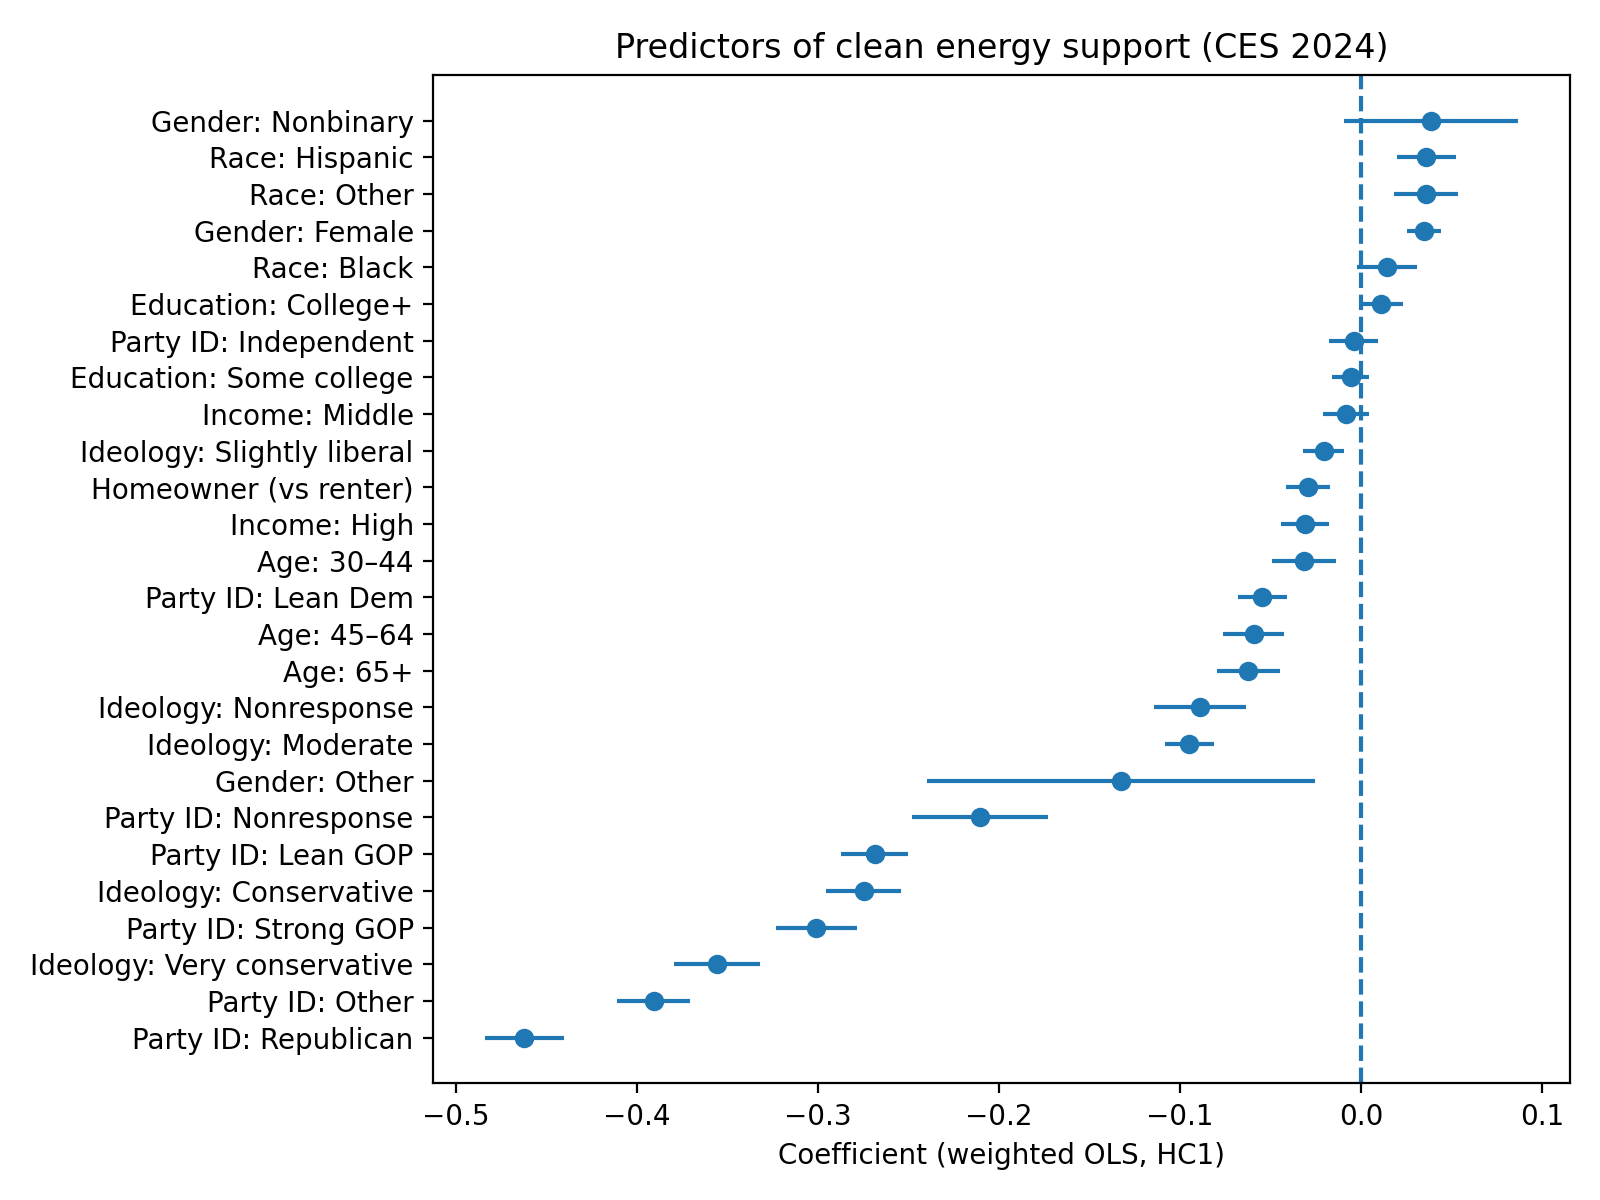
\includegraphics[keepaspectratio]{02_brief_files/figure-pdf/cell-4-output-1.png}}

As expected from the ``common sense'' view of how views of such policies
are distributed, party identification and political ideology are the
strongest predictors of clean energy support. Moving from liberal to
conservative ideological categories is associated with large declines in
support, and partisan differences are substantial.

However, even after accounting for these political variables,
homeownership remains negatively associated with clean energy support.
The estimated effect is modest in magnitude (approximately −0.03 on a
0--1 scale), but statistically significant and comparable to or larger
than the effect of moving between income categories.

To facilitate interpretation, Table 1 presents a labeled regression
table with human-readable predictor names.

\begin{Shaded}
\begin{Highlighting}[]
\NormalTok{HTML(}\BuiltInTok{open}\NormalTok{(}\StringTok{"exports/tables/wls\_table\_labeled.html"}\NormalTok{).read())}
\end{Highlighting}
\end{Shaded}

\begin{longtable}[]{@{}llll@{}}
\caption{}\label{T_fad71}\tabularnewline
\toprule\noalign{}
Block & Predictor & Coef (HC1) & 95\% CI \\
\midrule\noalign{}
\endfirsthead
\toprule\noalign{}
Block & Predictor & Coef (HC1) & 95\% CI \\
\midrule\noalign{}
\endhead
\bottomrule\noalign{}
\endlastfoot
Class: Income / Education / Tenure & Income: High & -0.030700 &
{[}-0.0441, -0.0174{]} \\
Class: Income / Education / Tenure & Homeowner (vs renter) & -0.029300 &
{[}-0.0415, -0.0170{]} \\
Class: Income / Education / Tenure & Income: Middle & -0.008400 &
{[}-0.0211, 0.0043{]} \\
Class: Income / Education / Tenure & Education: Some college & -0.005700
& {[}-0.0162, 0.0047{]} \\
Class: Income / Education / Tenure & Education: College+ & 0.011100 &
{[}-0.0012, 0.0233{]} \\
Demographics & Gender: Other & -0.132500 & {[}-0.2397, -0.0253{]} \\
Demographics & Age: 65+ & -0.062100 & {[}-0.0796, -0.0447{]} \\
Demographics & Age: 45--64 & -0.059300 & {[}-0.0762, -0.0423{]} \\
Demographics & Age: 30--44 & -0.031400 & {[}-0.0489, -0.0139{]} \\
Demographics & Race: Black & 0.014300 & {[}-0.0024, 0.0311{]} \\
Demographics & Gender: Female & 0.034800 & {[}0.0255, 0.0442{]} \\
Demographics & Race: Other & 0.036000 & {[}0.0183, 0.0537{]} \\
Demographics & Race: Hispanic & 0.036100 & {[}0.0197, 0.0525{]} \\
Demographics & Gender: Nonbinary & 0.038900 & {[}-0.0091, 0.0870{]} \\
Politics: Ideology & Ideology: Very conservative & -0.356000 &
{[}-0.3798, -0.3322{]} \\
Politics: Ideology & Ideology: Conservative & -0.274800 & {[}-0.2957,
-0.2539{]} \\
Politics: Ideology & Ideology: Moderate & -0.094900 & {[}-0.1084,
-0.0813{]} \\
Politics: Ideology & Ideology: Nonresponse & -0.088800 & {[}-0.1144,
-0.0633{]} \\
Politics: Ideology & Ideology: Slightly liberal & -0.020600 &
{[}-0.0320, -0.0092{]} \\
Politics: Party ID & Party ID: Republican & -0.462300 & {[}-0.4840,
-0.4405{]} \\
Politics: Party ID & Party ID: Other & -0.390800 & {[}-0.4110,
-0.3706{]} \\
Politics: Party ID & Party ID: Strong GOP & -0.300900 & {[}-0.3231,
-0.2786{]} \\
Politics: Party ID & Party ID: Lean GOP & -0.268700 & {[}-0.2873,
-0.2500{]} \\
Politics: Party ID & Party ID: Nonresponse & -0.210500 & {[}-0.2481,
-0.1730{]} \\
Politics: Party ID & Party ID: Lean Dem & -0.054400 & {[}-0.0679,
-0.0409{]} \\
Politics: Party ID & Party ID: Independent & -0.004000 & {[}-0.0177,
0.0096{]} \\
\end{longtable}

Notably, high incomes are weakly associated with lower support, while
middle incomes show little difference relative to low incomes. In
addition, education's effects are small once political orientation is
controlled for. The homeowner coefficient remains negative net of all
controls.

These results indicate that housing tenure captures something distinct
from income and ideology, likely related to asset ownership, exposure to
energy costs, or perceived regulatory risk.

\subsection{Predicted Values: Visualizing the Tenure
Gap}\label{predicted-values-visualizing-the-tenure-gap}

To make these results more intuitive, Figure 3 plots predicted levels of
clean energy support across the ideological spectrum, holding other
covariates constant.

\begin{Shaded}
\begin{Highlighting}[]
\NormalTok{display(Image(filename}\OperatorTok{=}\StringTok{"exports/figures/predicted\_support\_ideo\_income.png"}\NormalTok{))}
\end{Highlighting}
\end{Shaded}

\pandocbounded{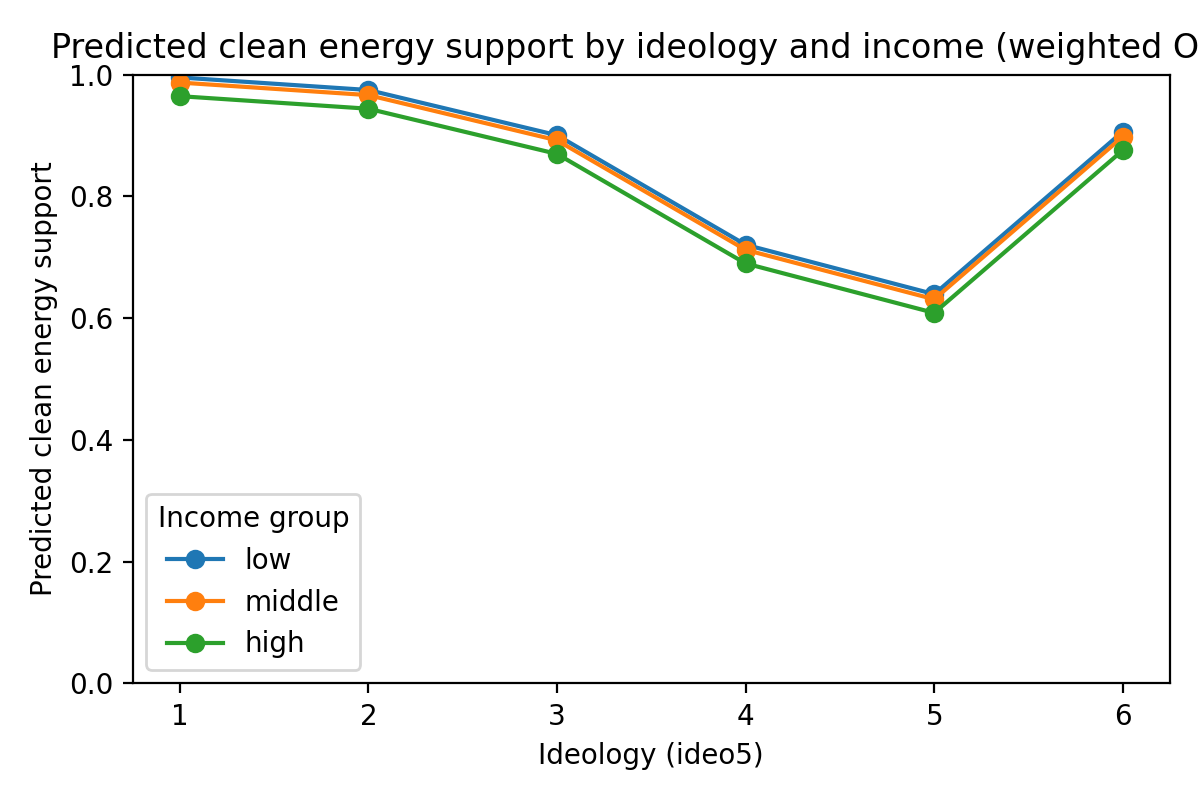
\includegraphics[keepaspectratio]{02_brief_files/figure-pdf/cell-6-output-1.png}}

This graphic suggests that, quite unsusprisingly, ideology strongly
structures climate attitudes, with steep declines in suport from liberal
to conservative positions. However, income differences are modest at
most ideological levels, and homeownership shifts the entire curve
downward, indicating lower support across ideological positions. In
other words, homeowners are less supportive of clean energy policies
even when they share similar ideological positions with renters.

\subsection{Interpretation and
Implications}\label{interpretation-and-implications}

Taken together, these findings suggest that support for clean energy
policy is shaped not only by ideology and partisanship, but also by
material position within the housing system. Homeownership appears to be
associated with lower support for environmental regulation in ways not
reducible to income or political identity.

One plausible interpretation is that homeowners face different perceived
costs and risks from climate and energy regulation, including concerns
about housing retrofits, energy prices, or property values. While the
CES cannot directly test these mechanisms, the results point to the
importance of considering tenure and asset exposure when analyzing
public opinion on climate policy.

More broadly, this analysis demonstrates that survey data, often
criticized for capturing only ``attitudes'',can still be used to study
structured differences linked to social position, especially when
variables are interpreted relationally rather than as isolated
preferences.

\subsection{Limitations and Next
Steps}\label{limitations-and-next-steps}

This analysis is descriptive and cross-sectional; therefore causal
interpretations should be avoided without further work. Additionally,
the clean energy support index weights all component items equally,
which may obscure percieved differences in the in the percieved impact
or importance of specific policies.

Future work could:

-Examine individual policy items as robustness checks

-Incorporate geographic context or energy cost measures

-Explore longitudinal changes in tenure and climate attitudes

Nonetheless, the present results provide clear evidence that housing
tenure is an underappreciated dimension of class relevant to
understanding support for climate friendly politics.

\subsection{View my GitHub repo for notes on methodology
here:}\label{view-my-github-repo-for-notes-on-methodology-here}

\href{https://github.com/bmdknndy/HomeOwnershipClimatePolicySupport}{GitHub}

To reproduce:

\begin{enumerate}
\def\labelenumi{\arabic{enumi}.}
\item
  run all DuckDB SQL scripts in sql/ folder
\item
  run notebooks/01\_analysis.ipynb
\item
  run report/brief.ipynb
\end{enumerate}

For additional details on methods, run
notebooks/03\_methods\_appendix.ipynb

\textbf{\emph{Brady Kennedy}}




\end{document}
